\section{Exact-Cover}
\subsection{Kundenanalyse}
Student Xaver Tecco soll im Rahmen einer Big-Data-Studienarbeit die Kunden einer gros- sen Shop-Website untersuchen und klassifizieren. Es steht eine grosse Zahl von binären Eigen- schaften zur Verfügung, zum Beispiel ob Kunden ein bestimmtes Produkt gekauft haben, oder ob ein Kunde nur im Dezember einkauft. Herr Tecco soll herausfinden, ob es eine Teilmenge von Kriterien derart gibt, dass jeder Kunde genau eine der Eigenschaften hat. Die Abgabe der Arbeit steht in zwei Tagen bevor, und er hat noch keinen funktionierenden Algorithmus. Muss er sich Sorgen machen?\\
\\
\textbf{Lösung}
Dieses Problem ist äquivalent mit dem bekanntermassen NP-vollständigen Problem EXACT-COVER:
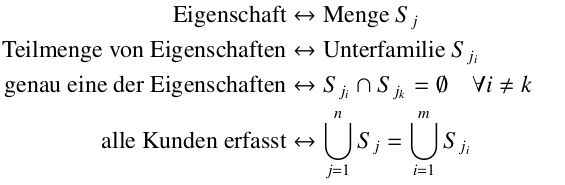
\includegraphics[width=\columnwidth]{img/exact-cover.png}

\subsection{Sehenswürdigkeiten}
Ein Tourist besucht ein fernes Land und kauft sich bei der Ankunft am Flughafen einen Führer, der all die zahlreichen Sehenswürdigkeiten enthält, die er gerne besuchen möchte. Er sagt sich, dass er seine Besichtigungspläne am besten so organisiert, dass er an jedem Tag eine Gruppe von Sehenswürdigkeiten besucht, die nahe beeinander liegen. Als nahe beeinander liegend klassifiziert er jeweils solche, die in kurzer Zeit mit öffentlichen Verkehrsmitteln erreichbar sind. Für jeden Tag seines Aufenthalts könnte er dann genau eine Gruppe von Sehenswürdig- keiten auswählen, so dass er am Ende alle gewünschten Sehenswürdigkeiten gesehen hat und keine zweimal besucht. Dank eines Sabbaticals war er zeitlich frei und stellte sich vor, seinen Aufenhalt nötigenfalls zu verlängern, sollte er mit seinen Besichtigungen nicht durchkommen. Nach einigen fehlgeschlagenen Versuchen, das Problem im Kopf zu lösen, setzt er sich in eine Caffeteria am Flughafen und arbeitet an dem Problem weiter. Er sagt sich, dass eine sorgfältige Planung durchaus einen ersten Tag ohne Besuch einer Sehenswürdigkeit wert ist. Als es dunkel wird ohne dass er eine Lösung gefunden hat, muss er sich eingestehen, dass das Problem doch nicht ganz einfach ist und beschliesst, am nächsten Morgen weiterzuarbeiten. Schliesslich geht nichts über eine sorgfältige Planung. Warum besteht die Gefahr, dass der arme Mann seine Heimreise antreten wird, ohne auch nur eine einzige Sehenswürdigkeit besucht zu haben?\\
\\
\textbf{Lösung}
Das beschriebene Problem BESICHTIGUNGS-PLANUNG ist das NP-vollständige Problem EXACT-COVER, für das es nach aktuellem Wissen keinen polynomiellen Algorithmus gibt. Die Menge U besteht aus allen Sehenswürdigkeiten des Führers. Die Teilmengen S j sind die Sehenswürdigkeiten, die der Tourist als nahe beeinander klassifiziert hat. Die Vereinigung $\bigcup_{j=1}^n S_j$ umfasst die Sehenswürdigkeiten, die der Tourist in seine Planung einbezogen hat. Gesucht ist eine disjunkte Teilfamilie $S_{j_i}$ , die alle Sehenswürdigkeiten umfasst, also
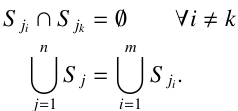
\includegraphics[width=\columnwidth/2]{img/sehenswuerdigkeiten.png}